\chapter{研究目的}
前述の通り、IJJ素子の特性を調べるため、40GHz以上で共振周波数の調整が可能な空洞共振器の設計が目的である。過去の研究成果を元に詳しい目標を整理する。

\section{昨年度の研究結果}
昨年度は、空洞共振器の大きさと誘電体を挿入した際の共振周波数を調べていた。\cite{わたなべ}
その結果誘電体を挿入することで、共振周波数を下げられることがわかった。

\vspace{10 mm}

\begin{figure}[h]
  \begin{center}
    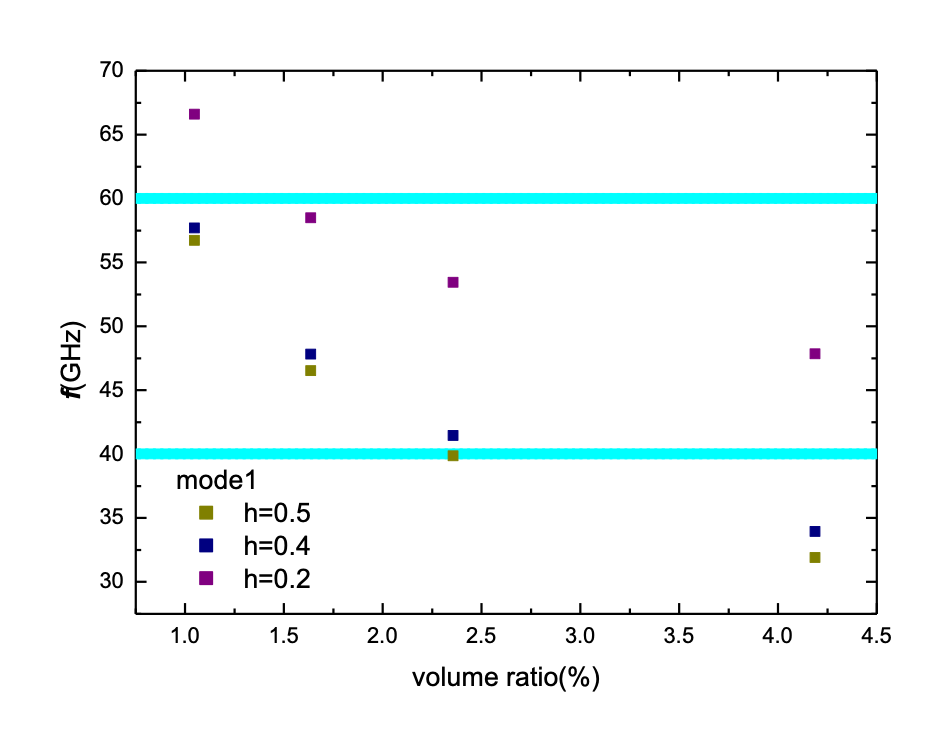
\includegraphics[width=12cm]{./image/watanabe.png}
    \caption{昨年度の誘電体挿入時の共振周波数変化}
    \label{fig:Watanabe}
  \end{center}
\end{figure}

\section{昨年度の課題}
昨年度の研究により、誘電体を挿入した際に共振周波数が下がることが観測されたが、以下の理由により実用的な(実現可能な)モデルとは言えなかった。


\subsection*{共振周波数の調整方法}
昨年度使用していた誘電体の誘電率は100程度であり、マイクロメータを使用して共振周波数を調整したとしても、細く共振周波数を変化させられる仕様ではなかった。



また、シミュレーションを実施したパターンが方形、円筒形の共振器の場合、誘電体が方形、円筒形の場合程度で検証したパターン数が少なく、具体的にどのようにして、精度よく共振周波数を調整するのかが不明瞭であった。

\subsection*{外界との結合方法}
空洞共振器は単体で共振現象を起こすものではなく、必ず外部からマイクロ波を入射し、外界からの入力の電磁場と共振させたいモードの電磁場を結合する必要がある。今回は、外界と共振器の電磁場を結合させるために、同軸ケーブルを使用する。昨年度作成していたモデルでは、一辺の長さが1mm程度であり、直径が2mm程度の同軸ケーブルでは接続することができなかった。

\subsection*{試料の設置位置が不明瞭}
資料の設置一は内部電場の分布から決定するが、昨年度の結果では、誘電体挿入時内部の電磁場がどのような分布になるのかが明らかになっていなかったため、試料の設置位置も決定できなかった。

\section{本研究の目的}
昨年度の研究結果を受けて、改めて整理すると、

\begin{itemize}
  \item 誘電体による共振周波数の変化の傾向を明らかにする
  \item 同軸ケーブルとの接続を想定したモデル
  \item 誘電体挿入時の電場変化を考慮して試料設置位置を決定する
\end{itemize}

以上3点を満たした、共振周波数40GHz以上で調整可能な、実用的な空洞共振器の設計を行うことが本研究の目標である。
% また、調整精度に関しては現時点では不明であるため、
